\documentclass[12pt]{article}

\usepackage{graphicx}
\usepackage{fancyhdr}
\usepackage{biblatex}
\usepackage{rotating}
\usepackage{xcolor}
\usepackage{listings}
\usepackage{indentfirst}
\usepackage{float}
\usepackage{longtable}
\usepackage[margin=1in]{geometry}
\usepackage[hyphens]{url}

\bibliography{bib.bib}
\setlength{\parskip}{\baselineskip}%

\lstset{basicstyle=\ttfamily,
  showstringspaces=false,
  commentstyle=\color{red}
  keywordstyle=\color{blue}
}

\title{CS 751: Introduction to Digital Libraries - Assignment 4}
\author{Jessica McConnell}
\date{\today}

\begin{document}
\sloppy
\maketitle

\section{Q1}

I again used the boilerpipe application suggested in the Assignment 3 powerpoint by Christian Kohlschütter. \cite{Kohlschütter:2011:boilerpipe}

\subsection{Picking Files}
Using the files in my `GoodFiles' file from Assignment 3, I redownloaded all the URIs using a script modified from Assignment 1 called `getAll.sh'

\subsection{Running Files}
I modified my java program from Assignment 3 and named it `A4.java'.  It takes all the file names for the URIs in the `GoodFiles' file and runs the downloaded html for the URI through boilerpipe using the ArtifactExtract function.  I compiled and ran my java file with the following 2 commands:

\begin{lstlisting}[language=bash]
javac -d . -cp .:../boilerpipe-1.2.0/boilerpipe-1.2.0.jar: - 
../boilerpipe-1.2.0/nekohtml-1.9.13.jar:../boilerpipe-1.2.0/ - 
xerces-2.4.0.jar:../boilerpipe-1.2.0/* A4.java

java -cp .:../boilerpipe-1.2.0/boilerpipe-1.2.0.jar: - 
../boilerpipe-1.2.0/nekohtml-1.9.13.jar:../boilerpipe - 
-1.2.0/xerces-2.4.0.jar:../boilerpipe-1.2.0/* A4
\end{lstlisting}

I received FileNotFound exceptions on several files.  This must mean the web pages for those links do not exist any longer and were not downloaded using my `getAll.sh' script.

\subsection{Statistics}
The downloaded pages were 58 days apart. I downloaded the first set of pages on February 10, 2015. The second set of pages was downloaded on April 9, 2015.

I modified my `uniqueWords.py' script from Assigment 3 to get all unigrams, bigrams and trigrams for the old and new downloaded URI file. After that it performed set operations to find the Jaccard Distance for each.

To get the data for my Cumulative Distribution Function Graph I ran the following command for one word, two words and three words only changing the filename and which field I kept after the cut.

\begin{lstlisting}[language=bash]
atria:~/cs751/a4> python uniqueWords.py fileNames > wordDiff
atria:~/cs751/a4> grep wordDiff | cut -d',' -f1 | sort -n > sortedOneDiff
\end{lstlisting}

\begin{figure}[H]
    \centering
    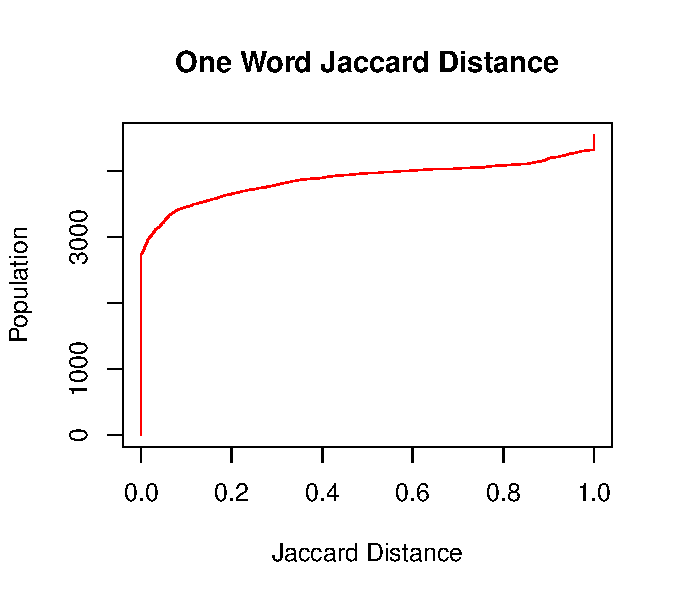
\includegraphics[scale=0.7]{oneDiff.pdf}
\end{figure}

\begin{figure}[H]
    \centering
    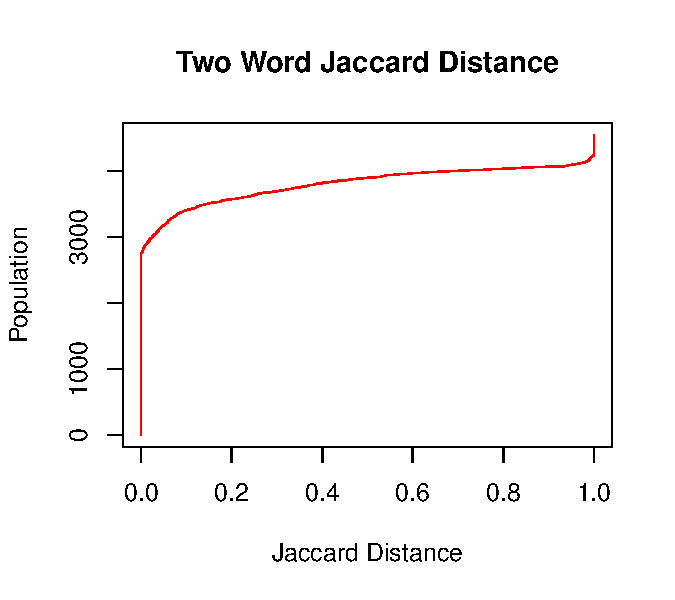
\includegraphics[scale=0.7]{twoDiff.pdf}
\end{figure}

\begin{figure}[H]
    \centering
    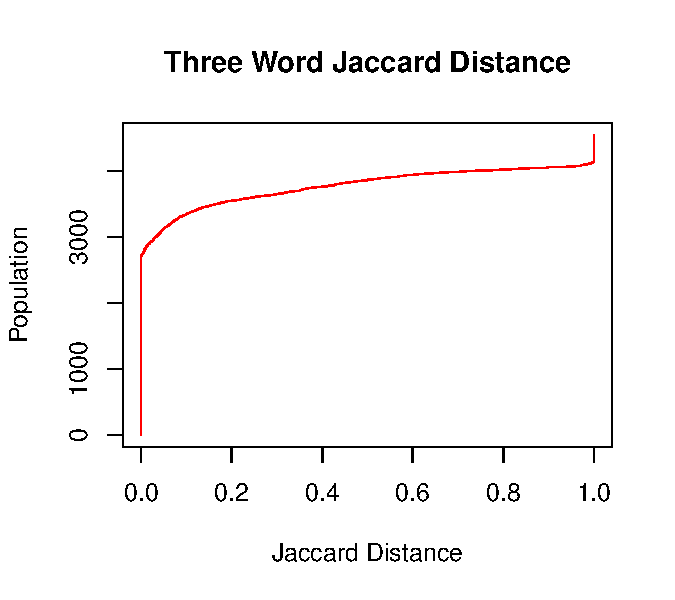
\includegraphics[scale=0.7]{threeDiff.pdf}
\end{figure}

\subsection{Range of Changes}
\url{https://www.pinterest.com/pin/115052965456448281?utm_content=buffere9579&utm_medium=social&utm_source=twitter.com&utm_campaign=buffer}\\
\begin{tabular}{|c|c|c|}
    \hline
    unigrams & bigrams & trigrams\\
    \hline
    0.571 & 0.800 & 0.889\\
    \hline
\end{tabular}

BEFORE:\\
There’s more to see...\\
Sign up to discover and save different things to try in 2015.\\
Continue 

AFTER:\\
There’s more to see...\\
30 billion ideas to discover, and only 45 seconds to sign up!\\
Continue

EXPLANATION: The Jaccard Distance is close to one because the two URI files are almost completely different. The unigrams Jaccard Distance is still fairly low because many of the words were repeated; however, they were in a different order making the bigrams and trigrams higher.


\url{http://ask.fm/JulienneMaeMarcellana/answer/113886611337}\\
\begin{tabular}{|c|c|c|}
    \hline
    unigrams & bigrams & trigrams\\
    \hline
    0.000 & 0.000 & 0.000\\
    \hline
\end{tabular}

BEFORE:\\
Report\\
Do you believe in love?\\
The question is who doesn't. Jk. To be honest, I'm not really into the grandiose aspect of love. Let's just say that I dwell on the commitment side of any relationship and not much on the romantic part.

AFTER:\\
Report\\
Do you believe in love?\\
The question is who doesn't. Jk. To be honest, I'm not really into the grandiose aspect of love. Let's just say that I dwell on the commitment side of any relationship and not much on the romantic part.

EXPLANATION: Nothing changed between these two.

\url{http://www.ebay.com/itm/like/111579677690?item=111579677690&lgeo=1NEW&vectorid=229466&rmvSB=true}\\
\begin{tabular}{|c|c|c|}
    \hline
    unigrams & bigrams & trigrams\\
    \hline
    0.080 & 0.088 & 0.105\\
    \hline
\end{tabular}

BEFORE:\\
End of add to list layer
 
FREE Expedited Shipping\\
Import charges:\\
(amount confirmed at checkout) To be provided at checkout  help icon for Shipping - opens a layer\\
This amount includes applicable customs duties, taxes, brokerage and other fees. This amount is subject to change until you make payment. For additional information, see the Global Shipping Program terms and conditions- opens in a new window or tab This amount includes applicable customs duties, taxes, brokerage and other fees. This amount is subject to change until you make payment. If you reside in an EU member state besides UK, import VAT on this purchase is not recoverable. For additional information, see the Global Shipping Program terms and conditions- opens in a new window or tab\\
No additional import charges on delivery\\
Delivery:\\
On or before Tue. Apr. 14 to 23529 Estimated by eBay FAST 'N FREE  help icon for Estimated delivery date - opens a layer\\
Items showing "eBay FAST 'N FREE" have an estimated delivery time of 4 business days or less. eBay FAST 'N FREE is our proprietary method of estimating delivery times based on the buyer's proximity to the item location, the shipping service selected, the seller's shipping history, and other factors. Delivery times may vary, especially dURIng peak periods.\\
Returns:\\
Seller does not offer returns. You are covered by the eBay Money Back Guarantee - opens in a new window or tab if you received an item that is not as described in the listing.\\
Guarantee:\\
Get the item you ordered or get your money back.\\
Covers your purchase price and original shipping.\\
28 items similar to NEW DUO Victoria's Secret Wild Rasp/Straw Juiced Berry Beauty Rush Mist \& Lotion\\

AFTER:\\
End of add to list layer
 
FREE Standard Shipping\\
Import charges:\\
(amount confirmed at checkout) To be provided at checkout  help icon for Shipping - opens a layer\\
This amount includes applicable customs duties, taxes, brokerage and other fees. This amount is subject to change until you make payment. For additional information, see the Global Shipping Program terms and conditions- opens in a new window or tab This amount includes applicable customs duties, taxes, brokerage and other fees. This amount is subject to change until you make payment. If you reside in an EU member state besides UK, import VAT on this purchase is not recoverable. For additional information, see the Global Shipping Program terms and conditions- opens in a new window or tab\\
No additional import charges on delivery\\
Delivery:\\
On or before Mon. Feb. 16 to 23529 Estimated by eBay FAST 'N FREE  help icon for Estimated delivery date - opens a layer\\
Items showing "eBay FAST 'N FREE" have an estimated delivery time of 4 business days or less. eBay FAST 'N FREE is our proprietary method of estimating delivery times based on the buyer's proximity to the item location, the shipping service selected, the seller's shipping history, and other factors. Delivery times may vary, especially dURIng peak periods.\\
Returns:\\
Seller does not offer returns. You are covered by the eBay Money Back Guarantee - opens in a new window or tab if you received an item that is not as described in the listing.\\
Guarantee:\\
Get the item you ordered or get your money back.\\
Covers your purchase price and original shipping.\\
28 items similar to NEW DUO Victoria\&\#039;s Secret Wild Rasp/Straw Juiced Berry Beauty Rush Mist \&amp; Lotion\\

EXPLANATION: There was very little change between the two files. All I was able to find different was that the shipping type changed from "FREE Expedited Shipping" to "FREE Standard Shipping".

\url{http://thetruth24.com/post/107421}\\
\begin{tabular}{|c|c|c|}
    \hline
    unigrams & bigrams & trigrams\\
    \hline
    1.000 & 1.000 & 1.000\\
    \hline
\end{tabular}

BEFORE:\\
News\\
Balaclava-clad raider pulls 2ft sword on betting shop staff\\
Police have released CCTV footage of the moment a balaclava-clad raider    threatens betting shop staff with a 2ft sword.\\
The offender struck a computer screen and knocked over displays at Coral    bookmakers opposite Burnley FC's Turf Moor ground as he terrorised two    employees with his demands for cash.\\
He then jumped over the counter and stole between £150 and £200 from the till    of the shop before it is thought he made off.\\
The incident took place at about 8.45pm on Monday, July 21 last year.\\
The raider is described as white, 5ft 10in, with a slim build, who was wearing    a grey tracksuit top with a logo on the top of the hood and dark tracksuit    bottoms.\\
He spoke with a local accent, police added.\\
DC Dave Greenwood of Pennine CID, said: "This was a violent and    aggressive attack which left two members of staff terrified and fearful for    their own safety.\\
"It has been some time since the initial incident but we remain    determined to identify the man responsible and hope that someone who views    the footage may hold important information about his identity."\\
30/01/2015 15:06     by: Telegraph

AFTER:

EXPLANATION: The second time I tried to pull the page we were unable to.  Since we couldn't pull the page down the second time they are completely different making a Jaccard Distance of 1 for all.

\section{Q2}
\subsection{Getting Timemaps}
I used the server hosted by the ODU CS department mementoproxy.cs.odu.edu to get my timemaps.  I wrote a bash script named `getTimeMaps.sh' to go through my list of unique URIs and curl the timemap URL.

\subsection{Counting Mementos}
I then ran the below bash command to search for all instances of `rel="memento"' for each individual URI.

\begin{lstlisting}[language=bash]
for item in `ls'; do 
  echo $item $(cat $item | cut -d`,' -f1- | 
  grep `rel="memento"' | wc -l); done > mementoToURI
\end{lstlisting}

\begin{figure}[H]
    \centering
    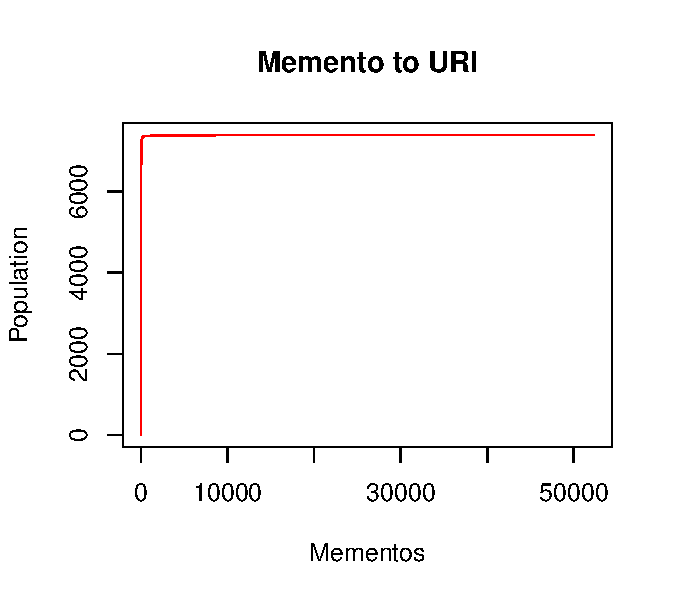
\includegraphics[scale=0.7]{mementoCount.pdf}
\end{figure}

From the data I have concluded that many of my URIs were not very popular. I made this conclusion because of the fact that I had so many URIs that had no recorded mementos. 

\section{Q3}
\subsection{Picking URIs}
I used my file I created named mementoToURI that gave me the count of mementos I had based on the URI.  Using this I started with all mementos that had exactly 20 mementos and moved up until I reached 20 total URIs that met all the requirements.  I did throw out some potential URIs if I already had a previous version of the beginning.  For example, most youtube and facebook URIs began with the same few set of mementos.  After I already had one of these in my URI list I did not add any more to my URI list.

\subsection{Getting the mementos}
I created a bash script named `getMementos.sh' that downloaded all the mementos.  I then copied and altered the `A4.java' program I wrote to use boilerpipe on all of the downloaded mementos. Each URIs set of mementos started at 0 for original. Each subsequent downloaded memento was saved as a file incremented by 1.  Therefore file 4 was 5 mementos after the original memento was taken.

\subsection{Data}
I copied and altered my `uniqueWords.py' script to get all unigrams for the original memento.  It then went on to get all the unigrams in each subsequent memento.  To get the Jaccard distance I got the intersection and union of the original unigrams and subsequent unigrams individually for each file.  All distances were recorded in the file `jaccard' in the folder for the URI.

\subsection{Graph Creation}
I created an Rscript file named `jaccard.R' that took two command line arguments to create multiple graphs.  The exact command I ended up using to create all my graphs is below:

\begin{lstlisting}[language=bash]
for folder in `cat ../mementoThroughTime/uris`; do 
    echo $folder; 
    file="../mementoThroughTime/"$folder"/jaccard"; 
    Rscript jaccard.R $file $folder.pdf;
done
\end{lstlisting}

\subsection{Graphs}

URI Number 106:\\
\begin{figure}[H]
    \centering
    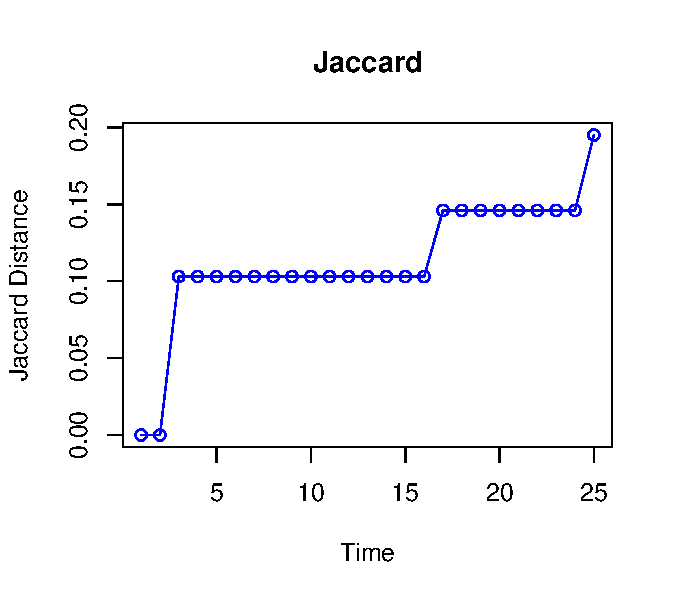
\includegraphics[scale=0.7]{106.pdf}
\end{figure}

URI Number 1628:\\
\begin{figure}[H]
    \centering
    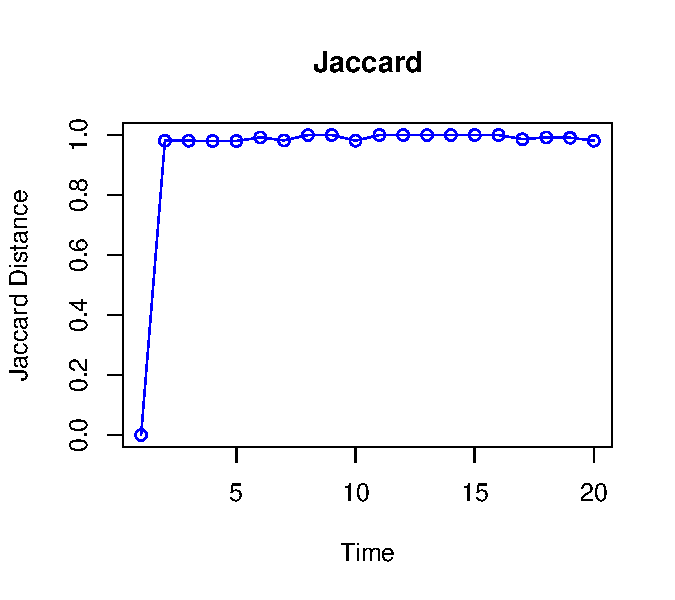
\includegraphics[scale=0.7]{1628.pdf}
\end{figure}

URI Number 21:\\
\begin{figure}[H]
    \centering
    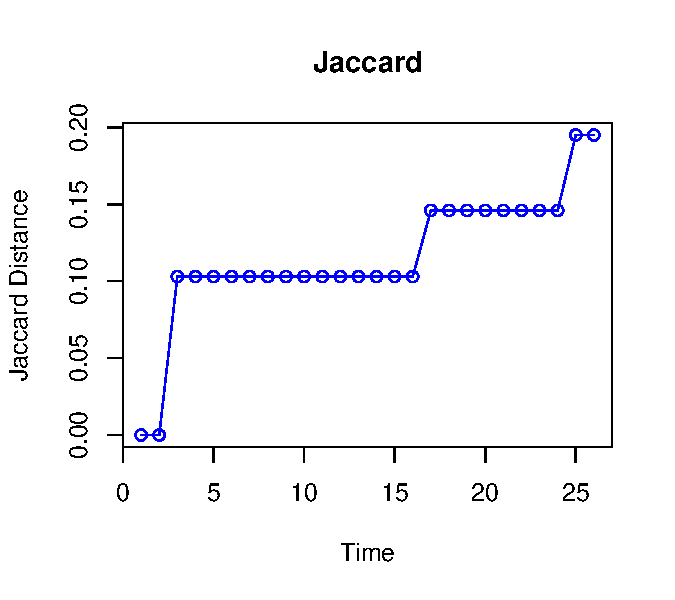
\includegraphics[scale=0.7]{21.pdf}
\end{figure}

URI Number 2452:\\
\begin{figure}[H]
    \centering
    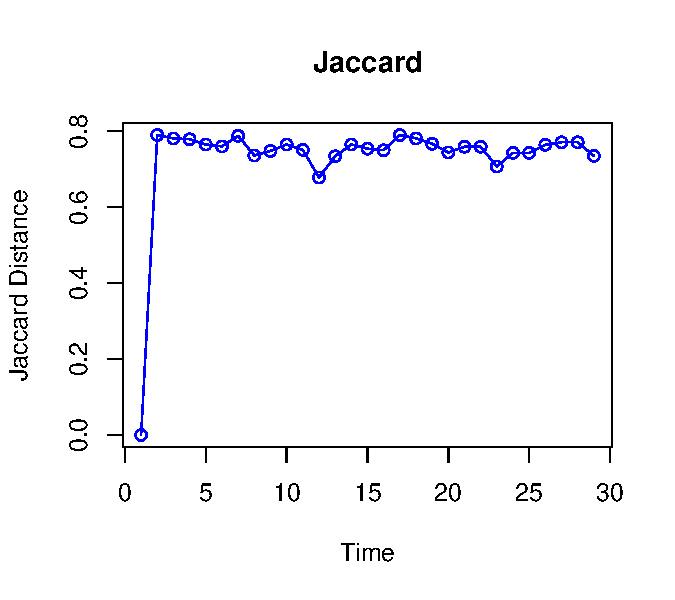
\includegraphics[scale=0.7]{2452.pdf}
\end{figure}

URI Number 3948:\\
\begin{figure}[H]
    \centering
    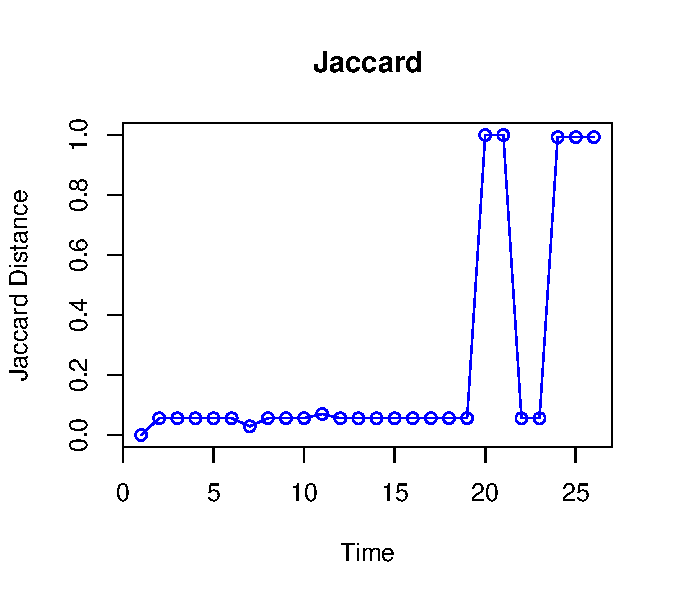
\includegraphics[scale=0.7]{3948.pdf}
\end{figure}

URI Number 4253:\\
\begin{figure}[H]
    \centering
    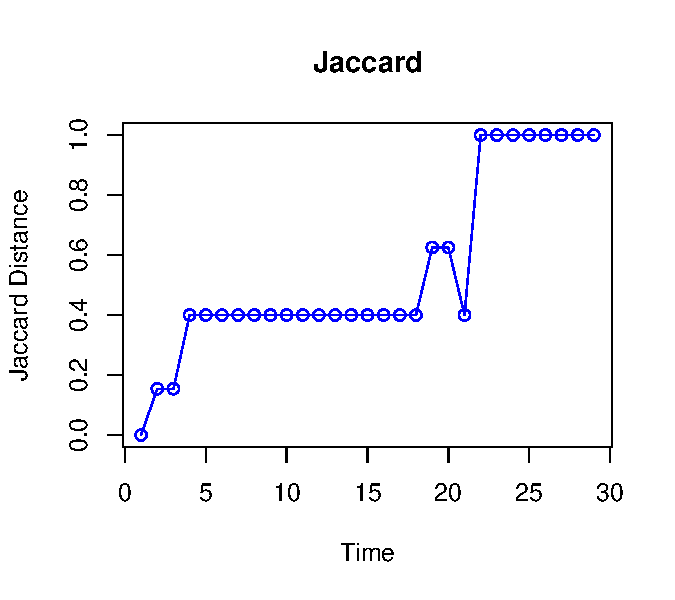
\includegraphics[scale=0.7]{4253.pdf}
\end{figure}

URI Number 4255:\\
\begin{figure}[H]
    \centering
    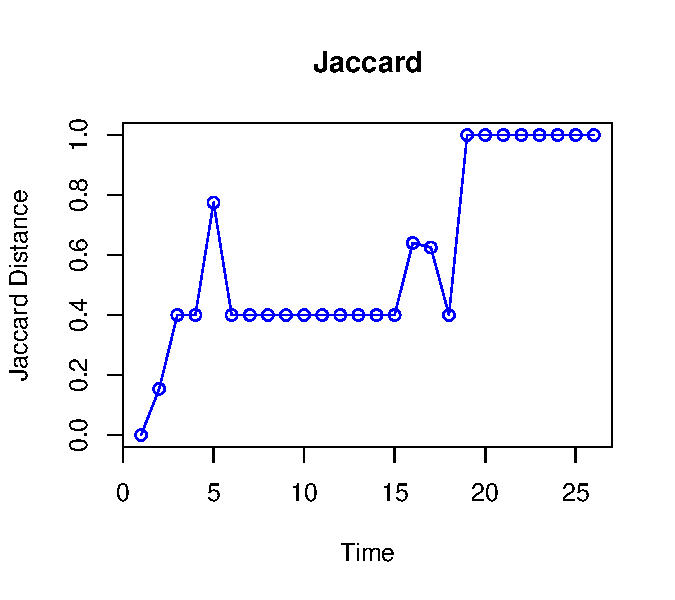
\includegraphics[scale=0.7]{4255.pdf}
\end{figure}

URI Number 4257:\\
\begin{figure}[H]
    \centering
    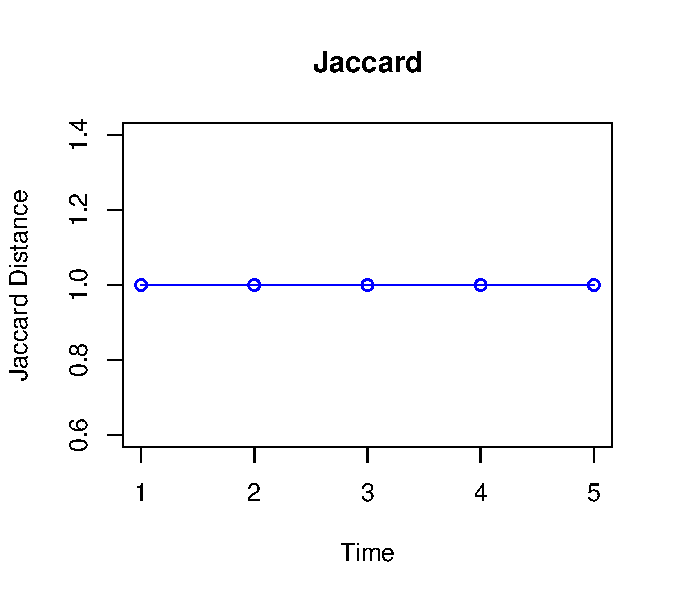
\includegraphics[scale=0.7]{4257.pdf}
\end{figure}

URI Number 4271:\\
\begin{figure}[H]
    \centering
    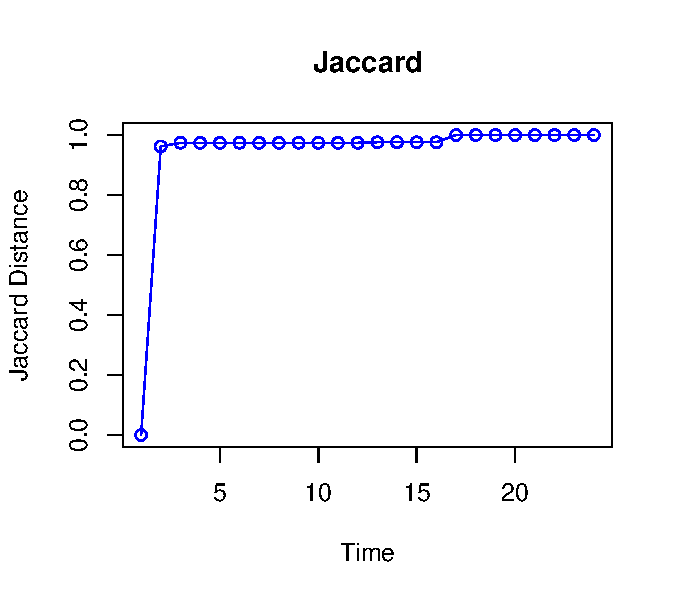
\includegraphics[scale=0.7]{4271.pdf}
\end{figure}

URI Number 4708:\\
\begin{figure}[H]
    \centering
    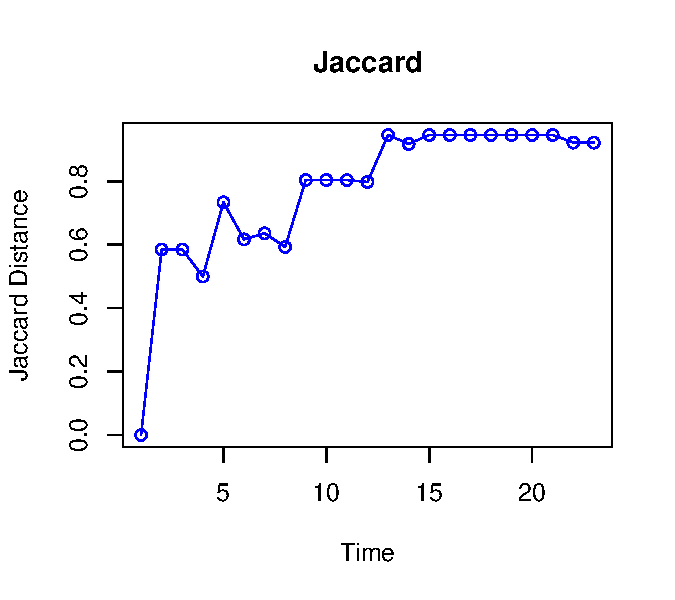
\includegraphics[scale=0.7]{4708.pdf}
\end{figure}

URI Number 4907:\\
\begin{figure}[H]
    \centering
    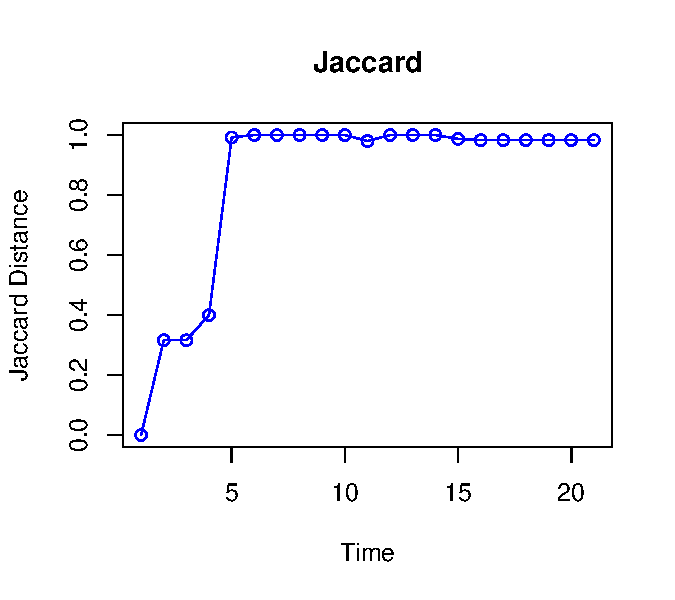
\includegraphics[scale=0.7]{4907.pdf}
\end{figure}

URI Number 4973:\\
\begin{figure}[H]
    \centering
    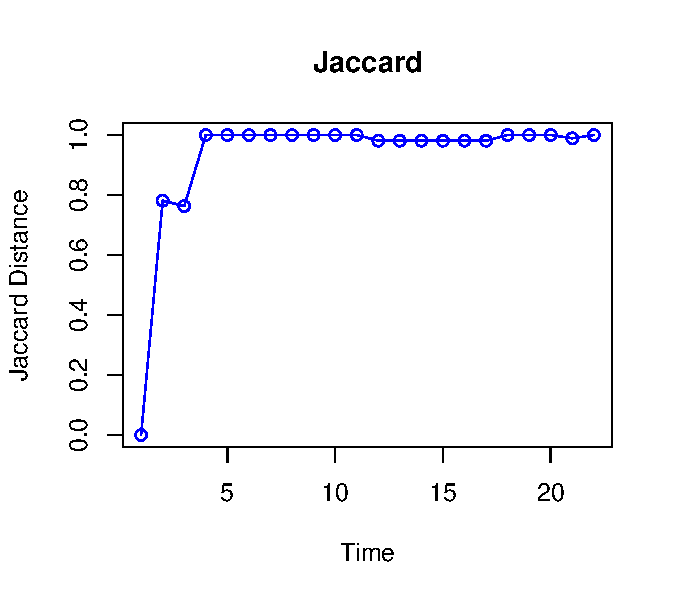
\includegraphics[scale=0.7]{4973.pdf}
\end{figure}

URI Number 5243:\\
\begin{figure}[H]
    \centering
    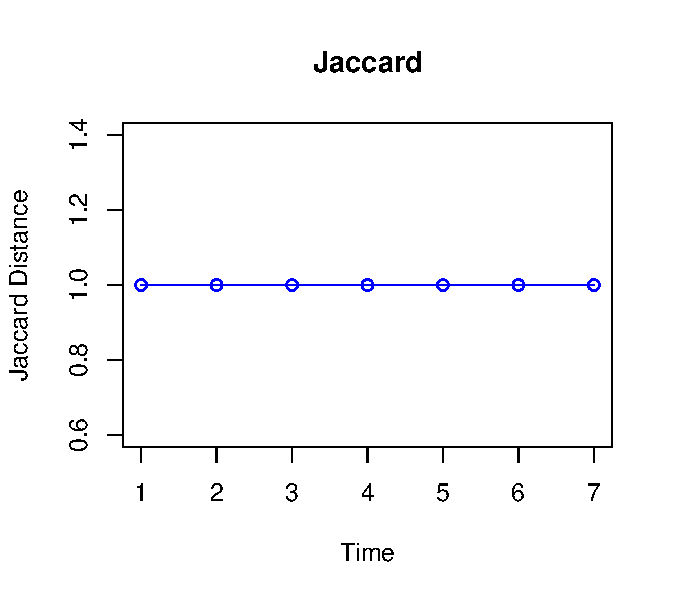
\includegraphics[scale=0.7]{5243.pdf}
\end{figure}

URI Number 528:\\
\begin{figure}[H]
    \centering
    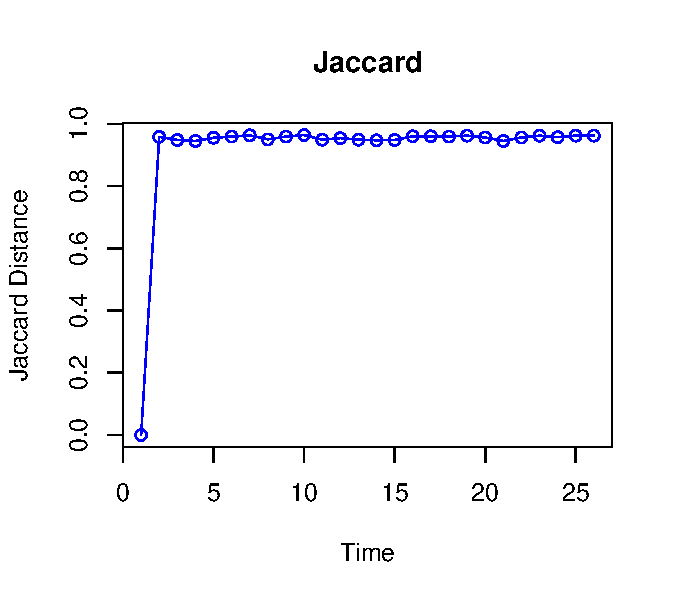
\includegraphics[scale=0.7]{528.pdf}
\end{figure}

URI Number 5383:\\
\begin{figure}[H]
    \centering
    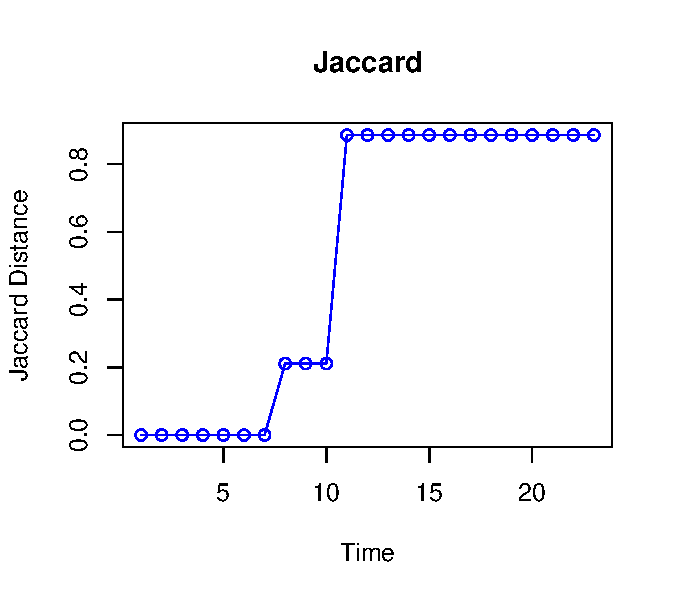
\includegraphics[scale=0.7]{5383.pdf}
\end{figure}

URI Number 5761:\\
\begin{figure}[H]
    \centering
    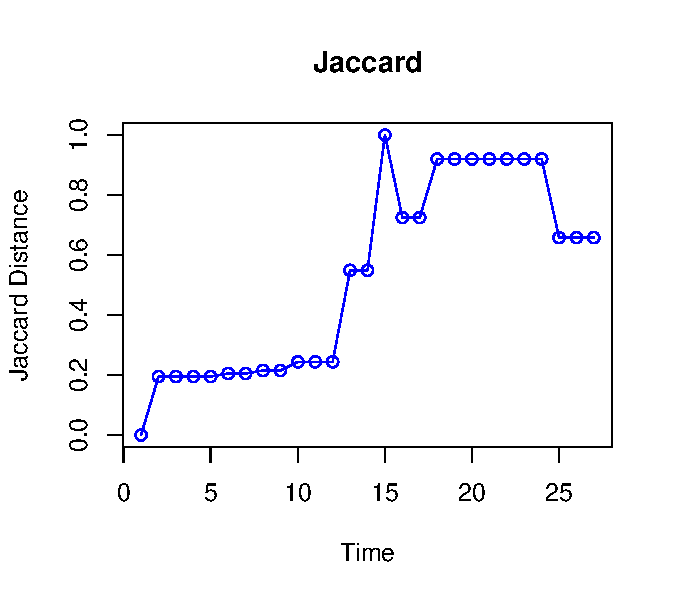
\includegraphics[scale=0.7]{5761.pdf}
\end{figure}

URI Number 583:\\
\begin{figure}[H]
    \centering
    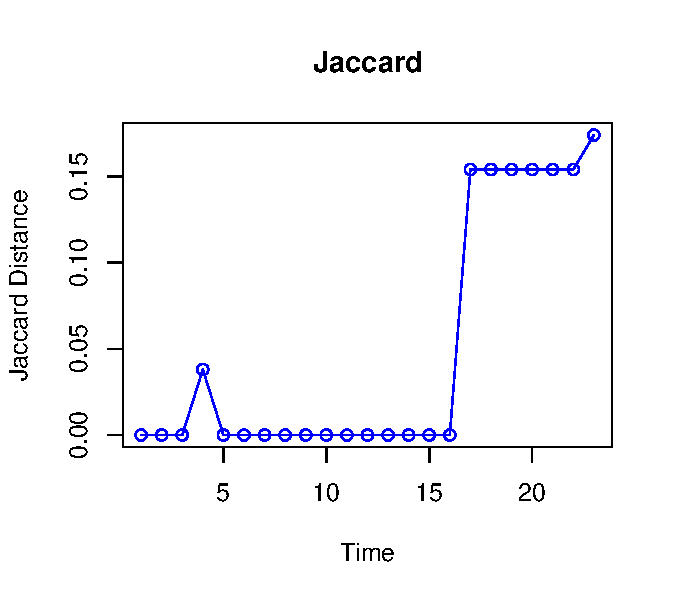
\includegraphics[scale=0.7]{583.pdf}
\end{figure}

URI Number 6377:\\
\begin{figure}[H]
    \centering
    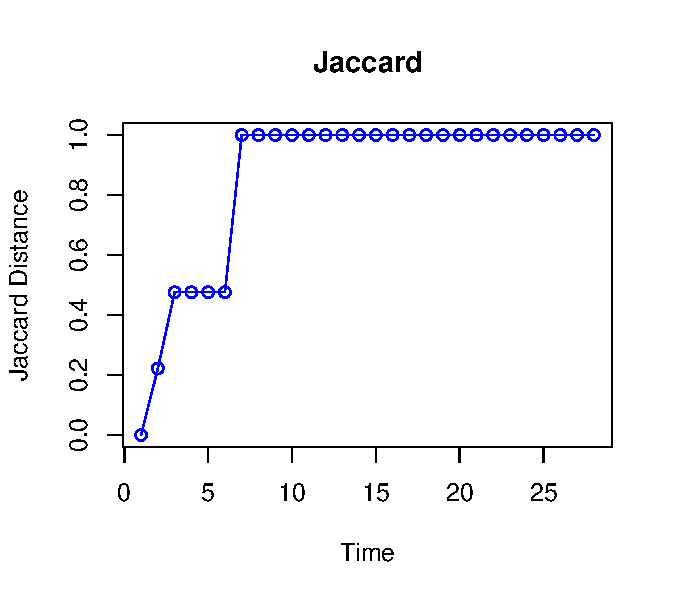
\includegraphics[scale=0.7]{6377.pdf}
\end{figure}

URI Number 6838:\\
\begin{figure}[H]
    \centering
    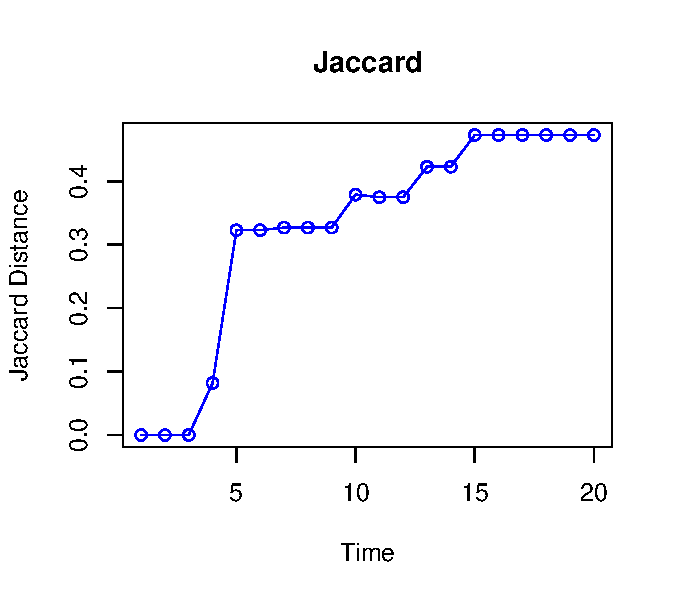
\includegraphics[scale=0.7]{6838.pdf}
\end{figure}

URI Number 759:\\
\begin{figure}[H]
    \centering
    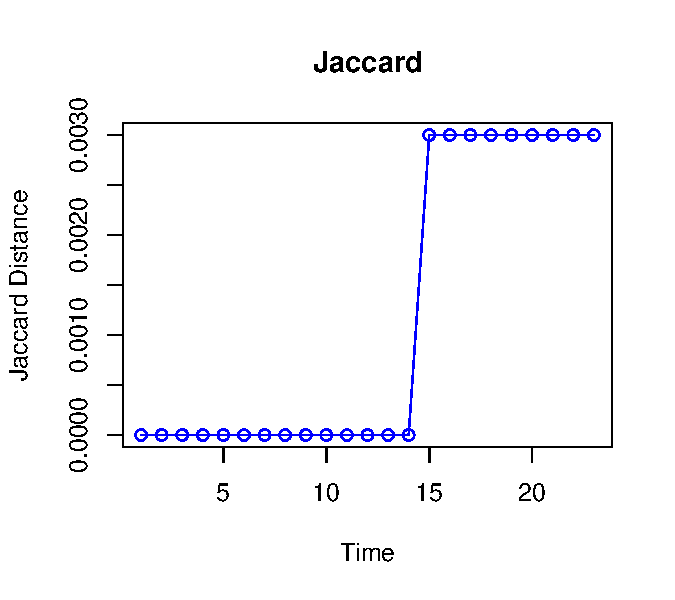
\includegraphics[scale=0.7]{759.pdf}
\end{figure}

\section{Extra Credit}
For this question I used the word "McDonnell" in my search. I picked this topic by browsing to the \url{www.pilotonline.com} website and choosing something that was on their front site. Each day I did a search (which resulted in much more than 1000 responses).  For the first day I took out the first 1000 tweets.  On each subsequent day I removed any responses I already had then took the next 1000 tweets.

I attempted to use the stream option, but it did not seem like my subject was actively being discussed.  I tried a few other topics that received similar results.  That is the reason I ended up going with my search method that I did.

All the walls, word clouds and geojson files can be found in the twarcs directory.

Creating the wall was a very simple process. The time it took to process/create the wall was pretty long though. This took nearly as much time as it did to search for the tweets from twitter. It is a great tool that shows all of the tweets in your json side-by-side with other tweets. It is especially interesting to see this when all the tweets have stuff in common.

A major issue I saw with the wall is that if I move the created .html file then none of the pictures correlating to the tweets would show up when replaying it in the browser.

The word cloud is especially interesting. It combines all the words in your selected set of tweets and shows them in a cloud format with varying sizes.  The sizes are dependent on the number of times the word was mentioned.

On the first day 2015-04-22 you see a lot of differently sized words all about the news story.

\begin{figure}[H]
    \centering
    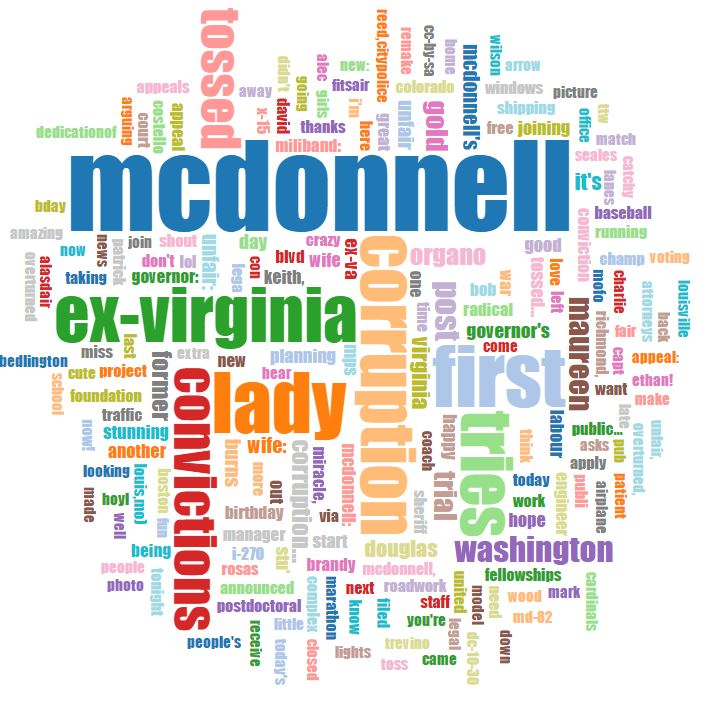
\includegraphics[scale=0.7]{20150422.JPG}
\end{figure}

On the last day 2015-04-26 there is only really one main word, McDonnell.  It seems like it started being less about the news story and more about other people with the last name McDonnell.

\begin{figure}[H]
    \centering
    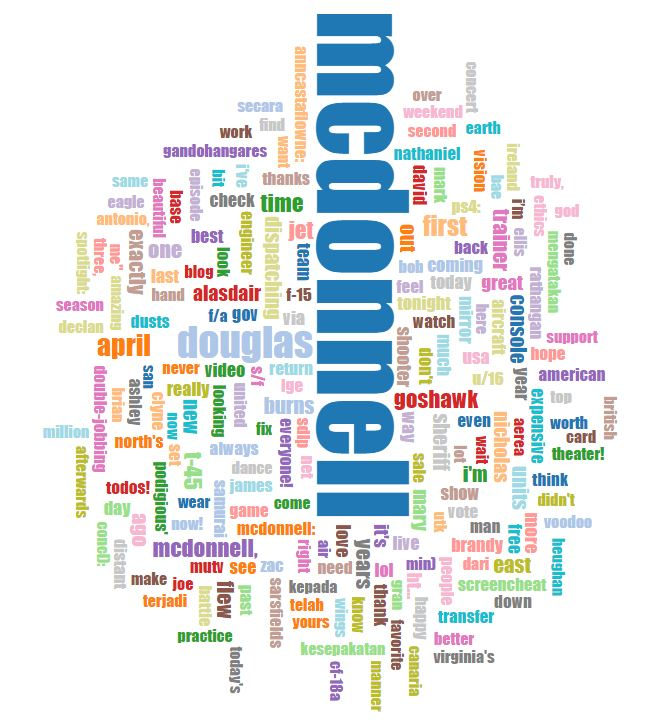
\includegraphics[scale=0.7]{20150426.JPG}
\end{figure}

A big issue I saw with the word cloud is that it kept punctuation at the end of the words.  This caused McDonnell, McDonnell:, McDonnell; and other variations to all be in the word cloud.  If they would have removed the punctuation, there could have been many different words with different sizes.



\printbibliography

\end{document}
